% !TeX root = skripta-konstitutivni-vztahy-materialu.tex
% !TeX lastmodified = 2019-04-01

\subsection{Přechod k~integrálnímu popisu viskoelastické látky}
Obecnější modely lze vytvořit rozšířením Kelvinova modelu.
\begin{figure}[H]
	\centering
	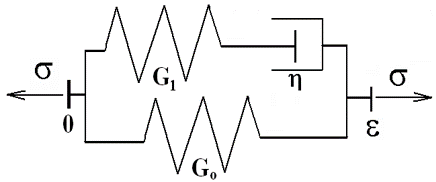
\includegraphics[width=0.4\linewidth]{standard-linear-solid}
	\caption{Standard linear solid}%todo změnit
\end{figure}

Jeho relaxace napětí je popsána rovnicí
\begin{equation}
	\sigma(t) = \varepsilon_0 \left[G_0 + G_1 \exp\! \left(-\frac{t}{\tau_\varepsilon} \right) \right] = \varepsilon_0 K(t),
\end{equation}
kde $K(t)$ je tzv. relaxační funkce.

Přidáváním dalších paralelních Maxwellových elementů do celkového počtu $n$ ji lze zobecnit do tvaru
\begin{equation}
	K(t) = \sum\limits_{i=0}^n G_i \exp\! \left(-\frac{t}{\tau_\varepsilon} \right) = \sum\limits_{i=0}^n G_i \exp\! \left(-t \nu_i\right),
\end{equation}
kde $\nu_i = \frac{1}{\tau_i}$ je relaxační frekvence $i$-tého Maxwellova prvku.

Vynesením závislosti amplitud $G_i$ jako funkce těchto frekvencí dostaneme diskrétní spektrum relaxačních funkcí.

\subsubsection{Diskrétní spektrum relaxačních funkcí}
Amplitudy jednotlivých členů $\alpha_i$ jsou zde normalizovány vůči celkovému modulu podle vztahu
\begin{equation}
	\alpha_i = \frac{G_i}{\sum_{i=0}^n G_i}
\end{equation}

\begin{figure}[H]
	\centering
	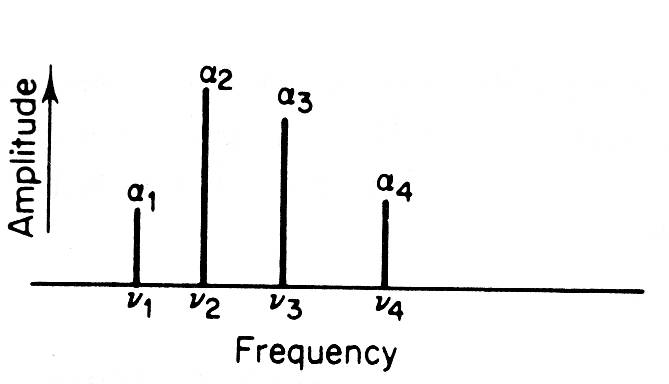
\includegraphics[width=0.4\linewidth]{spektrum-relaxacnich-funkci}
	\caption{Diskrétní spektrum relaxačních funkcí}
	\label{fig:spektrum-relaxacnich-funkci}
\end{figure}

\subsubsection{Boltzmannova formulace}
Nejobecnější formulace Boltzmannova vychází z~těchto předpokladů:
\begin{itemize}
	\item deformace je funkcí celé historie zatěžování až do vyšetřovaného času $t$,
	\item existuje proporcionalita (lineární závislost) mezi přírůstkem napětí $\diff \sigma(t)$ a~přírůstkem deformace $\diff \varepsilon(t)$,
	\item funkce $\sigma(t)$ je spojitá a~diferencovatelná.
\end{itemize}

Pak přírůstek napětí v~krátkém časovém intervalu $\diff \tau$ v~časovém okamžiku $\tau$ je $\left(\frac{\partial \sigma}{\partial \tau}\right) \diff \tau$.
Tento přírůstek napětí působí na těleso po celý zbývající časový interval $(t - \tau)$ a~k~přetvoření v~čase~$t$ přispívá přírůstkem $\diff \varepsilon(t)$, jehož závislost na přírůstku napětí v~čase je popsána funkcí $K$. Ta závisí na příslušném časovém intervalu $(t - \tau)$, takže platí
\begin{equation}
	\diff \varepsilon(t) = K(t - \tau) \frac{\partial \sigma}{\partial \tau} \diff \tau,
\end{equation}
kde funkce $K(t - \tau)$ je označována jako krípová nebo retardační funkce, resp. také relaxační funkce přetvoření.
Pokud položíme časový počátek do počátku pohybu (zatěžování), tak přetvoření lze určit integrací
\begin{equation}
	\varepsilon(t) = \int\limits_0^t K(t - \tau) \frac{\partial \sigma}{\partial \tau} \diff \tau.
\end{equation}

\subsubsection{Konvoluční integrál relaxační funkce}
Zaměníme-li roli napětí a~přetvoření (deformační zatěžování), pak dostaneme stejným postupem podobnou formulaci pro napětí:
\begin{equation}
	\sigma(t) = \int\limits_0^t C(t - \tau) \frac{\partial \varepsilon}{\partial \tau} \diff \tau,
\end{equation}
kde funkce $C(t - \tau)$ je relaxační funkce napětí. Zobrazení této funkce v~závislosti na čase nebo frekvenci představuje spojité relaxační spektrum.

Při začátku zatěžování v~čase $t = -\infty$, za předpokladu malých přetvoření i~posuvů, lze popsat závislost mezi napětími a~přetvořeními rozšířenými na tenzorové funkce závislé kromě času i~na prostorových souřadnicích bodu $\bm{x}(x_1, x_2, x_3)$ konvolučním integrálem 
\begin{equation}
	\sigma_{ij}(\bm{x}, t) = \int\limits_{-\infty}^t G_{ijkl}(\bm{x}, t - \tau) \frac{\partial \varepsilon_{kl}}{\partial \tau} (\bm{x}, \tau) \diff \tau,
\end{equation}
nebo jeho inverzním tvarem
\begin{equation}
	\varepsilon_{ij}(\bm{x}, t) = \int\limits_{-\infty}^t J_{ijkl}(\bm{x}, t - \tau) \frac{\partial \sigma_{kl}}{\partial \tau} (\bm{x}, \tau) \diff \tau,
\end{equation}
kde $G_{ijkl}$ je tenzorová relaxační funkce a~$J_{ijkl}$ je tenzorová krípová funkce.

V~praxi nelze integrovat od času $t = -\infty$, volíme tedy počátek časové osy v~okamžiku počátku pohybu, kdy těleso bylo nezatížené a~nedeformované.
Pak je např. konvoluční integrál pro napětí zredukován do tvaru
\begin{equation}
	\sigma_{ij}(\bm{x}, t) = \varepsilon_{kl}(\bm{x}, 0\!+) G_{ijkl}(\bm{x}, t)
	+ \int\limits_0^t G_{ijkl}(\bm{x}, t - \tau) \frac{\partial \varepsilon_{kl}}{\partial \tau} (\bm{x}, \tau) \diff \tau,
\end{equation}
kde $\varepsilon_{kl}(\bm{x}, 0+)$ je limita funkce $\varepsilon_{kl}(\bm{x}, t)$ pro $t \rightarrow 0$ zprava.
První člen na pravé straně rovnice představuje důsledek skokové změny přetvoření v~čase $t = 0$; podobný člen je třeba zavést v~každém časovém okamžiku, kdy funkce $\varepsilon_{kl}(\bm{x}, t)$ nemá derivaci (skokově se mění).

Zpracováno podle Funga\footnote{Y.C. Fung: Biomechanics. Springer, 1993.}.
